%%%%%%%%%%%%%%%%%%%%%%%%%%%%%%%%%%%%%%%%%%%%%%%%%%%%%%
% A Beamer template for University of Wollongong     %
% Based on THU beamer theme                          %
% Author: Qiuyu Lu                                   %
% Date: July 2024                                    %
% LPPL Licensed.                                     %
%%%%%%%%%%%%%%%%%%%%%%%%%%%%%%%%%%%%%%%%%%%%%%%%%%%%%%
% Customized for Sharif University of Technology     %
%%%%%%%%%%%%%%%%%%%%%%%%%%%%%%%%%%%%%%%%%%%%%%%%%%%%%%


\documentclass[serif, aspectratio=169]{beamer}
\usepackage{pgfplots} % Required for plotting
\pgfplotsset{compat=1.17} % Compatibility level
%\documentclass[serif]{beamer}  % for 4:3 ratio
\usepackage[T1]{fontenc} 
\usepackage{fourier} % see "http://faq.ktug.org/wiki/uploads/MathFonts.pdf" for other options
\usepackage{hyperref}
\usepackage{latexsym,amsmath,xcolor,multicol,booktabs,calligra}
\usepackage{graphicx,pstricks,listings,stackengine}
\usepackage{lipsum}
\usepackage{array}

\author{Ali Sharifi-Zarchi}
\title{Machine Learning (CE 40477)}
\subtitle{Fall 2024}
\institute{
    CE Department \\
    Sharif University of Technology
}
%\date{\small \today}
% \usepackage{UoWstyle}
\usepackage{SUTstyle}

% defs
\def\cmd#1{\texttt{\color{red}\footnotesize $\backslash$#1}}
\def\env#1{\texttt{\color{blue}\footnotesize #1}}
\definecolor{deepblue}{rgb}{0,0,0.5}
\definecolor{deepred}{RGB}{153,0,0}
\definecolor{deepgreen}{rgb}{0,0.5,0}
\definecolor{halfgray}{gray}{0.55}

\lstset{
    basicstyle=\ttfamily\small,
    keywordstyle=\bfseries\color{deepblue},
    emphstyle=\ttfamily\color{deepred},    % Custom highlighting style
    stringstyle=\color{deepgreen},
    numbers=left,
    numberstyle=\small\color{halfgray},
    rulesepcolor=\color{red!20!green!20!blue!20},
    frame=shadowbox,
}


\begin{document}

\begin{frame}
    \titlepage
    \vspace*{-0.6cm}
    \begin{figure}[htpb]
        \begin{center}
            
\includegraphics[keepaspectratio, scale=0.25]{pic/sharif-main-logo.png}
        \end{center}
    \end{figure}
\end{frame}

\begin{frame}    
\tableofcontents[sectionstyle=show,
subsectionstyle=show/shaded/hide,
subsubsectionstyle=show/shaded/hide]
\end{frame}

\section{Regularization \& Overfitting}

\subsection{Reviewing the Problem of Overfitting}

\begin{frame}{Reviewing the Problem of Overfitting}
    \begin{itemize} 
    
        \item \textbf{Recall from previous lectures:} Overfitting vs Underfitting
        
        \item \textbf{Overfitting:} Learning the underlying patterns and noise in the training data.
        \begin{itemize}
            \item High accuracy on training data but poor generalization on unseen data.
        \end{itemize}  

        \item \textbf{Underfitting:} The model is too simple to capture the patterns in the data.
        \begin{itemize}
            \item Poor performance on both training and test data.
        \end{itemize}

        \begin{figure}
                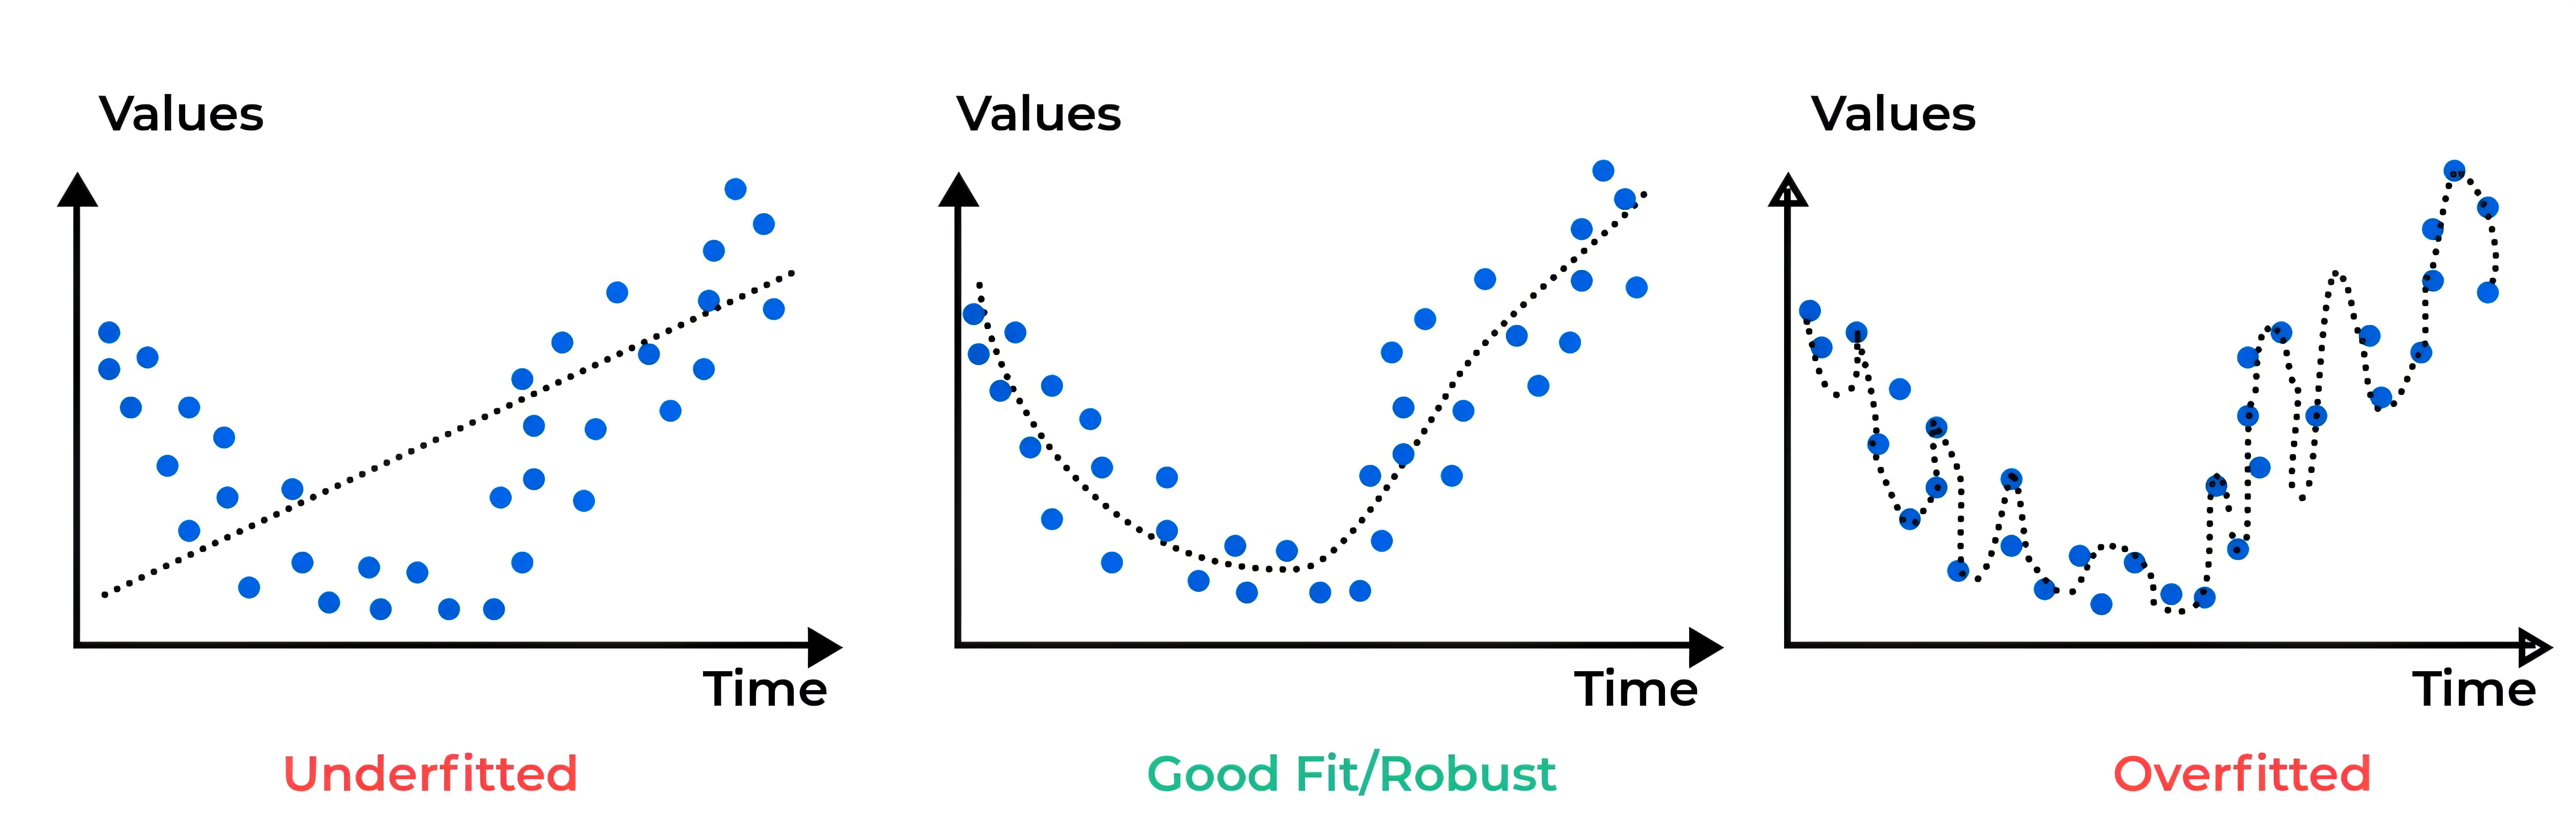
\includegraphics[width=0.9\textwidth]{pic/overfitting-vs-underfitting__AIE.png}
                \label{fig:overfitting-vs-underfitting}
        \end{figure}

    \end{itemize} 
\end{frame}


\subsection{Bias-Variance Tradeoff in Neural Networks}

\begin{frame}{Understanding the Bias-Variance Tradeoff}
    \begin{itemize}
        \item \textbf{Motivation:} 
            \begin{itemize}
                \item Balancing bias and variance is essential for training neural networks that \textbf{generalize} well to \textbf{unseen data}.
                \item In neural networks, model complexity can be increased with more layers or neurons, impacting both bias and variance.
            \end{itemize}
        \item \textbf{Core Concepts:} 
            \begin{itemize}
                \item \textbf{Bias:} Systematic error due to overly simplified assumptions.
                    \begin{itemize}
                        \item High-bias networks (e.g., shallow networks) may \textbf{underfit}, failing to capture complex patterns.
                    \end{itemize}
                \item \textbf{Variance:} Sensitivity to small changes in training data.
                    \begin{itemize}
                        \item High-variance networks (e.g., deep networks) may \textbf{overfit}, capturing noise in the data.
                    \end{itemize}
            \end{itemize}
    \end{itemize}
\end{frame}

\begin{frame}{Visualizing the Bias-Variance Tradeoff}
    \begin{itemize}
        \item \textbf{Tradeoff in Neural Networks:} Increasing layers and parameters can reduce bias but increase variance.
        \item \textbf{Finding the Balance:} \textbf{Regularization} methods help control this tradeoff by \textbf{adjusting model complexity}.
    \end{itemize}
\begin{figure}
        \centering
        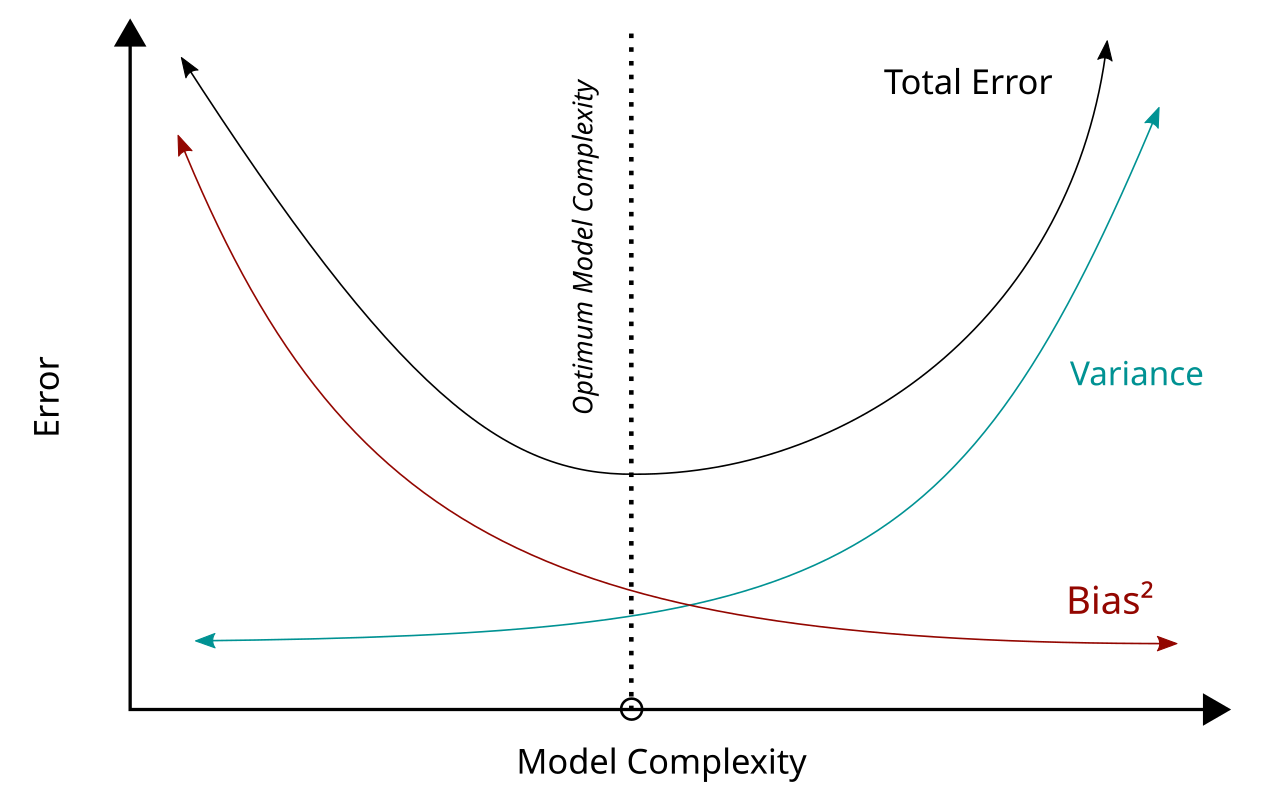
\includegraphics[width=0.4\textwidth]{pic/bv.png}
        \caption{Adapted from \href{en.wikipedia.org/wiki/Bias–variance_tradeoff}{Wikipedia}}
    \end{figure}
\end{frame}


\subsection{Inductive Bias in Neural Networks}

\begin{frame}{Inductive Bias in Neural Networks}
    \begin{itemize}
        \item \textbf{Definition:} 
            \begin{itemize}
                \item Inductive bias refers to \textbf{assumptions} embedded in the neural network's design to help it generalize to new, unseen data.
            \end{itemize}
        \item \textbf{Why it Matters:} 
            \begin{itemize}
            \item Translation invariance can hurt CNN performance when object position matters—a phenomenon known as the Picasso effect, where object parts are \textbf{present but misarranged}.
                \item Without inductive bias, networks would require \textbf{enormous data} to generalize effectively.
                \item In deep learning, architectural choices like convolutional layers (for spatial data) and recurrent layers (for sequential data) embody inductive biases.
            \end{itemize}
        \item \textbf{Classical Example:} 
            \begin{itemize}
                \item \textit{Occam's Razor}: Favoring simpler hypotheses (e.g., shallow networks) is an inductive bias that often aids generalization.
            \end{itemize}
    \end{itemize}
\end{frame}


\begin{frame}{Visualizing Inductive Bias}
\begin{figure}
        \centering
        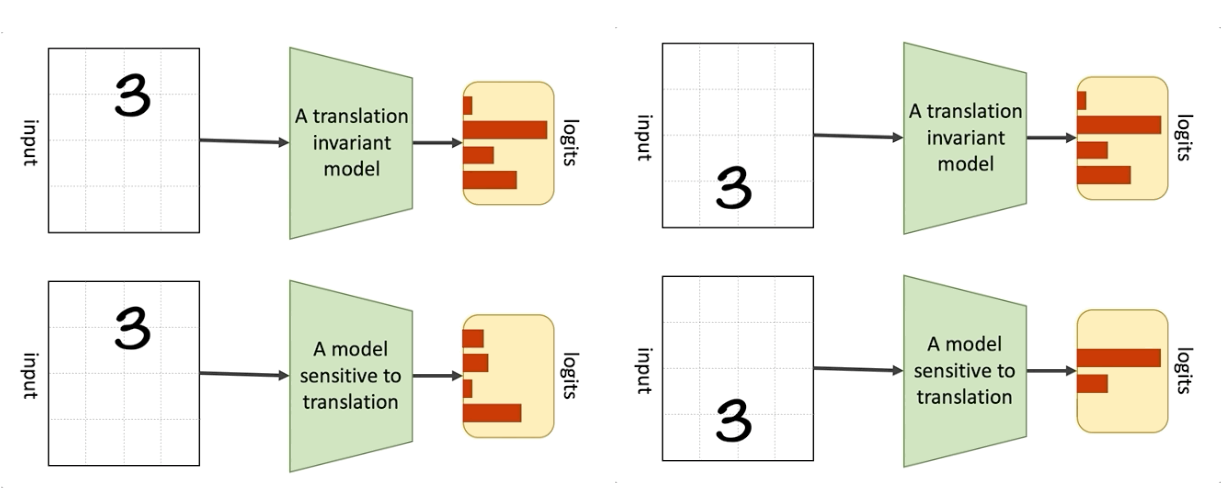
\includegraphics[width=0.85\textwidth]{pic/invariant-variant.png}
        \caption{Adapted from \href{https://samiraabnar.github.io/articles/2020-05/indist}{Distilling Inductive Biases}}
    \end{figure}
\end{frame}

\begin{frame}{Visualizing Inductive Bias}
\begin{figure}
        \centering
        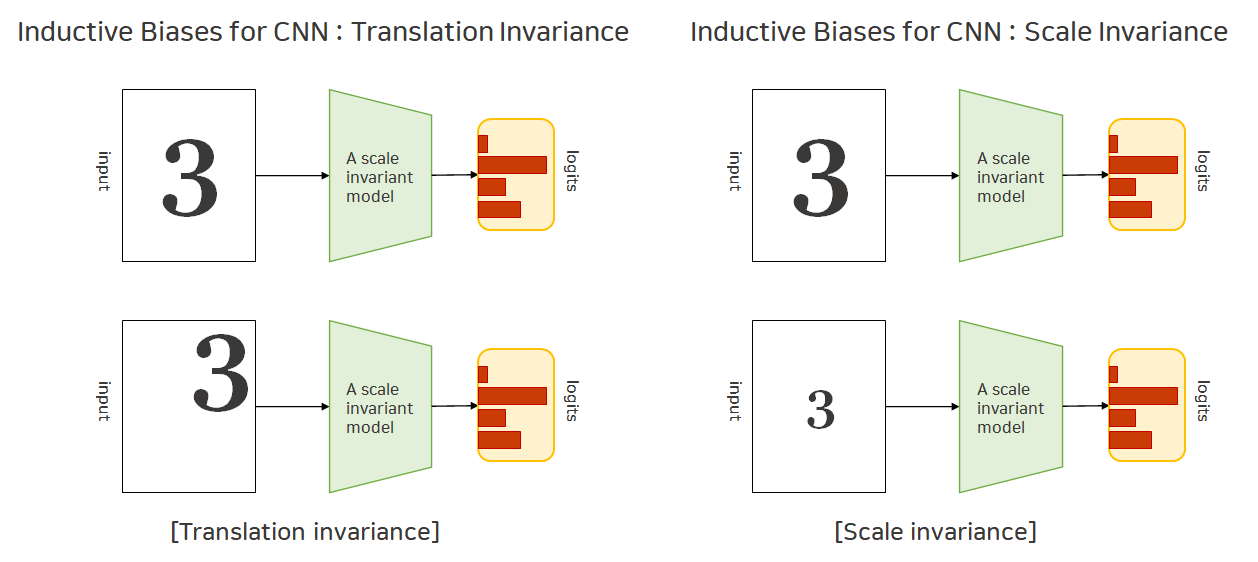
\includegraphics[width=0.85\textwidth]{pic/inductive.png}
        \caption{Adapted from \href{https://velog.io/@euisuk-chung/Paper-Review-Transferring-Inductive-Bias-Through-Knowledge-Distillation-33}{Transferring Inductive Bias Through Knowledge Distillation}}
    \end{figure}
\end{frame}


\begin{frame}{Visualizing Inductive Bias}
A drawing of how inductive biases can affect models' preferences to converge to different local minima. The inductive biases are shown by colored regions (green and yellow) which indicates regions that models prefer to explore.
\begin{figure}
        \centering
        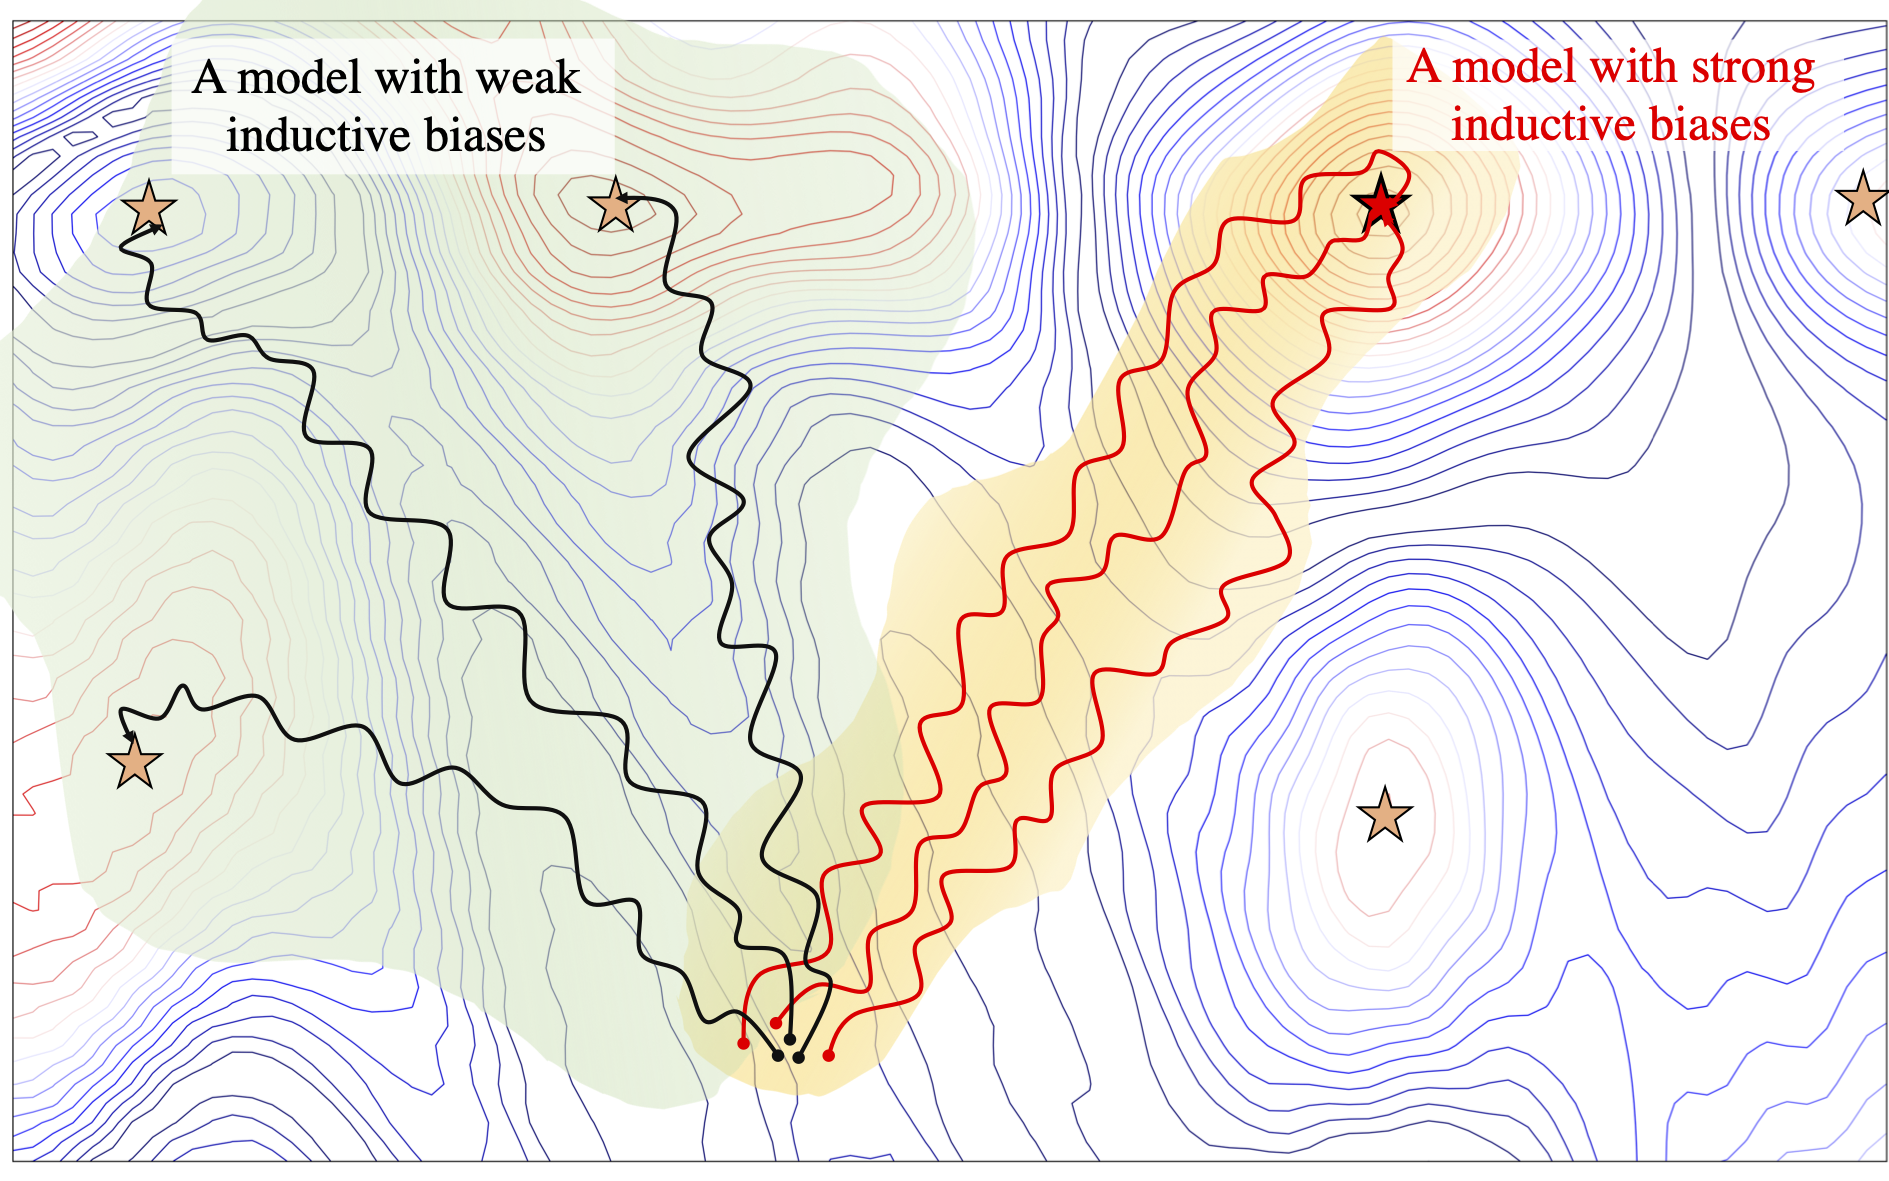
\includegraphics[width=0.5\textwidth]{pic/inductive_bias_distilation_example_1.png}
        \caption{Adapted from \href{https://samiraabnar.github.io/articles/2020-05/indist}{Distilling Inductive Biases}}
    \end{figure}
\end{frame}


\begin{frame}{Types of Inductive Bias in Neural Networks}
    \begin{itemize}
        \item \textbf{Convolutional Neural Networks (CNNs):} Designed with \textbf{locality and translation-invariance bias}. \\
              \textit{Example:} CNNs excel in image classification because nearby pixels often share related features.
              
        \item \textbf{Recurrent Neural Networks (RNNs):} Designed with \textbf{temporal continuity} bias, making them suitable for sequential data. \\
              \textit{Example:} RNNs work well for time series and natural language processing, where current information depends on previous data points.
              
        \item \textbf{Transformer Models:} Use attention mechanisms to capture \textbf{dependencies across positions} in data, embodying a flexible bias suitable for diverse tasks. \\
                            \textit{Example:} Transformers are highly effective in language modeling and tasks requiring understanding of long-range dependencies.

    \end{itemize}
\end{frame}


\begin{frame}{Adaptive Inductive Bias in Neural Networks}
    \begin{itemize}
        \item \textbf{Bias Shifting During Training:}
            \begin{itemize}
                \item Neural networks can adapt inductive bias as they learn, \textbf{dynamically adjusting} feature extraction layers.
            \end{itemize}
        \item \textbf{Implications in Transfer Learning:}
            \begin{itemize}
                \item Pre-trained networks on large datasets (e.g., ImageNet) carry learned inductive biases that can be \textbf{fine-tuned for specific applications}.
            \end{itemize}
        \item \textbf{Example in Practice:}
            \begin{itemize}
                \item Transfer learning in medical imaging, where pre-trained CNNs learn \textbf{domain-specific biases with limited labeled data}.
            \end{itemize}
    \end{itemize}
\end{frame}




\subsection{Regularization in Neural Networks}

\begin{frame}{Regularization in Neural Networks}
        \begin{itemize}
            \item \textbf{Goal:} Prevent overfitting.
            \item \textbf{Key Idea:} Favor simpler models to avoid fitting noise in the data.
        \end{itemize}

    \begin{figure}
        \centering
        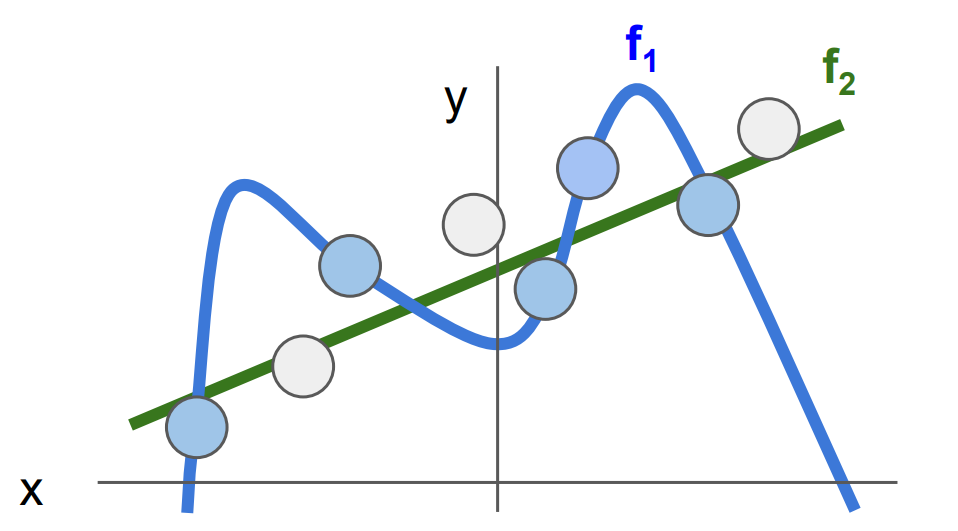
\includegraphics[width=0.5\textwidth]{pic/Regularization-intuition.png}
        \caption{Regularization prevents overfitting by avoiding fitting noise in the data.}
        \label{fig:Regularization-intuition}
    \end{figure}
\end{frame}


\begin{frame}{Regularization in Neural Networks}
    
\begin{equation}
J_\lambda(w) = \underbrace{J(w)}_{{\substack{\vphantom{\text{Prevent the model}} \\ \text{\textcolor{green} {\textbf{Data loss}}: Model predictions} \\ \text{should match training data}}}} + \underbrace{\lambda R(w)}_{{\substack{\vphantom{\text{Prevent the model}} \\ \text{\textcolor{green} {\textbf{Regularization}}: Prevent the model} \\ \text{from doing \textit{too} well on training data}}}}
\end{equation}


\end{frame}

\subsection{Key Regularization Techniques}
\begin{frame}{Key Regularization Techniques}
    \begin{itemize}[<+-| alert@+>] % stepwise alerts

            \item L1 (Lasso): Sparse weights, feature selection
                \begin{equation}
                    \text{L1 Regularization} = \lambda \sum_{j=1}^{m} |w_j|
                \end{equation}

            \item L2 (Ridge): Adds a penalty for large weights to the loss function
                \begin{equation}
                    \text{L2 Regularization} = \lambda \sum_{j=1}^{m} w_j^2 =
                    \lambda \textbf{W}^T\textbf{W}
                \end{equation}

            \item Elastic Net (L1 + L2): Combines both L1 and L2 penalties, where $\beta$ controls the balance between L1 and L2 regularization.

                \begin{equation}
                    \text{Elastic net Regularization} =\lambda \sum_{j=1}^{m} (\beta|w_j| + \frac{1-\beta}{2} w_j^2)
                \end{equation}
            
    \end{itemize}
\end{frame}

\begin{frame}{Key Regularization Techniques}
\begin{itemize}[<+-| alert@+>]

    \item \textbf{Lasso Regression (L1 Regularization):} Ideal for feature selection by setting some coefficients to zero.
    \begin{itemize}
        \item \textbf{Example:} Predicting house prices with many features. Lasso simplifies the model by focusing on key predictors (e.g., location, size).
        \item \textbf{Application:} Useful in NLP, where it identifies significant words by reducing others to zero.
    \end{itemize}
    
    \item \textbf{Ridge Regression (L2 Regularization):} Suitable when all features contribute meaningfully, minimizing overfitting without eliminating features.
    \begin{itemize}
        \item \textbf{Example:} Medical research using gene expression data, where every feature holds predictive power.
        \item \textbf{Application:} Ideal for multicollinear data, like predicting product sales with multiple correlated predictors.
    \end{itemize}
    
    \item \textbf{Elastic Net (L1 + L2):} Balances feature selection and generalization, effective with high feature correlation.
    \begin{itemize}
        \item \textbf{Example:} Financial models where predictors are correlated. Elastic Net combines Lasso’s selection with Ridge’s handling of multicollinearity.
    \end{itemize}
    
\end{itemize}
\end{frame}

\begin{frame}{Key Regularization Techniques}
\begin{table}[]
    \centering
    \begin{tabular}{|p{4cm}|p{4cm}|p{4cm}|}
        \hline
        \textbf{Characteristic} & \textbf{Ridge Regression} & \textbf{Lasso Regression} \\ \hline
        \textbf{Penalty Type} & L2 (squared coefficient magnitudes) & L1 (absolute coefficient magnitudes) \\ \hline
        \textbf{Coefficient Shrinkage} & Shrinks coefficients without setting to zero & Can shrink coefficients exactly to zero \\ \hline
        \textbf{Feature Selection} & Retains all features & Selects features by setting some to zero \\ \hline
        \textbf{Solution Path} & Coefficients generally non-zero & Many coefficients can be zero \\ \hline
        \textbf{Model Complexity} & Includes all features, higher complexity & Simplifies model by excluding features \\ \hline
    \end{tabular}
    \caption{Comparison of Ridge and Lasso Regression Techniques}
    \label{tab:ridge_vs_lasso}
\end{table}
\end{frame}

\begin{frame}{Key Regularization Techniques}
\begin{table}[]
    \centering
    \begin{tabular}{|p{4cm}|p{4cm}|p{4cm}|}
        \hline
        \textbf{Impact on Prediction} & Good for multicollinear data & Reduces model complexity, aiding high-dimensional data \\ \hline
        \textbf{Interpretability} & Less interpretable; all features retained & More interpretable; excludes irrelevant features \\ \hline
        \textbf{Best for} & When all features are relevant & When identifying key features among many \\ \hline
        \textbf{Bias-Variance Tradeoff} & Adds bias, reduces variance & Similar to Ridge, but with higher bias from exclusion \\ \hline
        \textbf{Computation} & Faster without feature selection & Slightly slower due to feature selection \\ \hline
    \end{tabular}
    \caption{Comparison of Ridge and Lasso Regression Techniques}
    \label{tab:ridge_vs_lasso}
\end{table}
\end{frame}


\begin{frame}{Key Regularization Techniques}

            \begin{figure}
                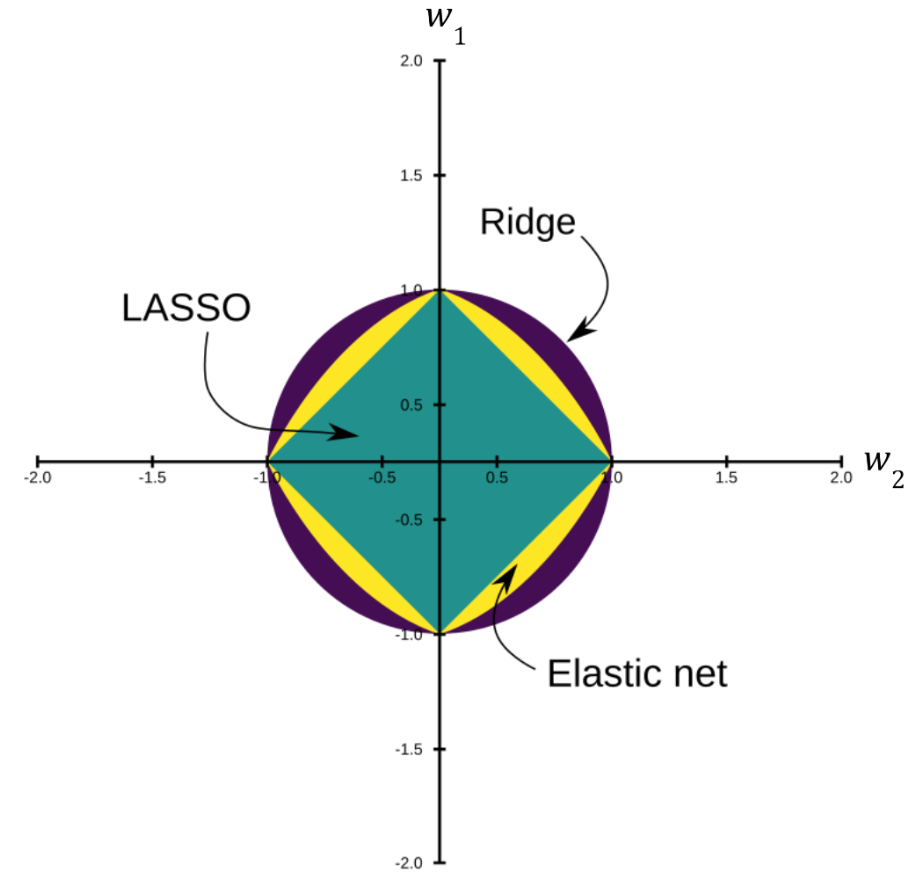
\includegraphics[width=0.4\textwidth]{pic/Regularization.png}
                 \caption{Lasso, Ridge, and Elastic net Comparision}
                \label{fig:Regularization}
            \end{figure}

\end{frame}

\begin{frame}{Key Regularization Techniques}
    \begin{itemize}

            \item Early Stopping
            \begin{itemize}
                \item Stops training when the validation loss stops improving.
                \item Prevents overfitting by avoiding excessive training beyond the optimal point.
            \end{itemize}

            \begin{figure}
                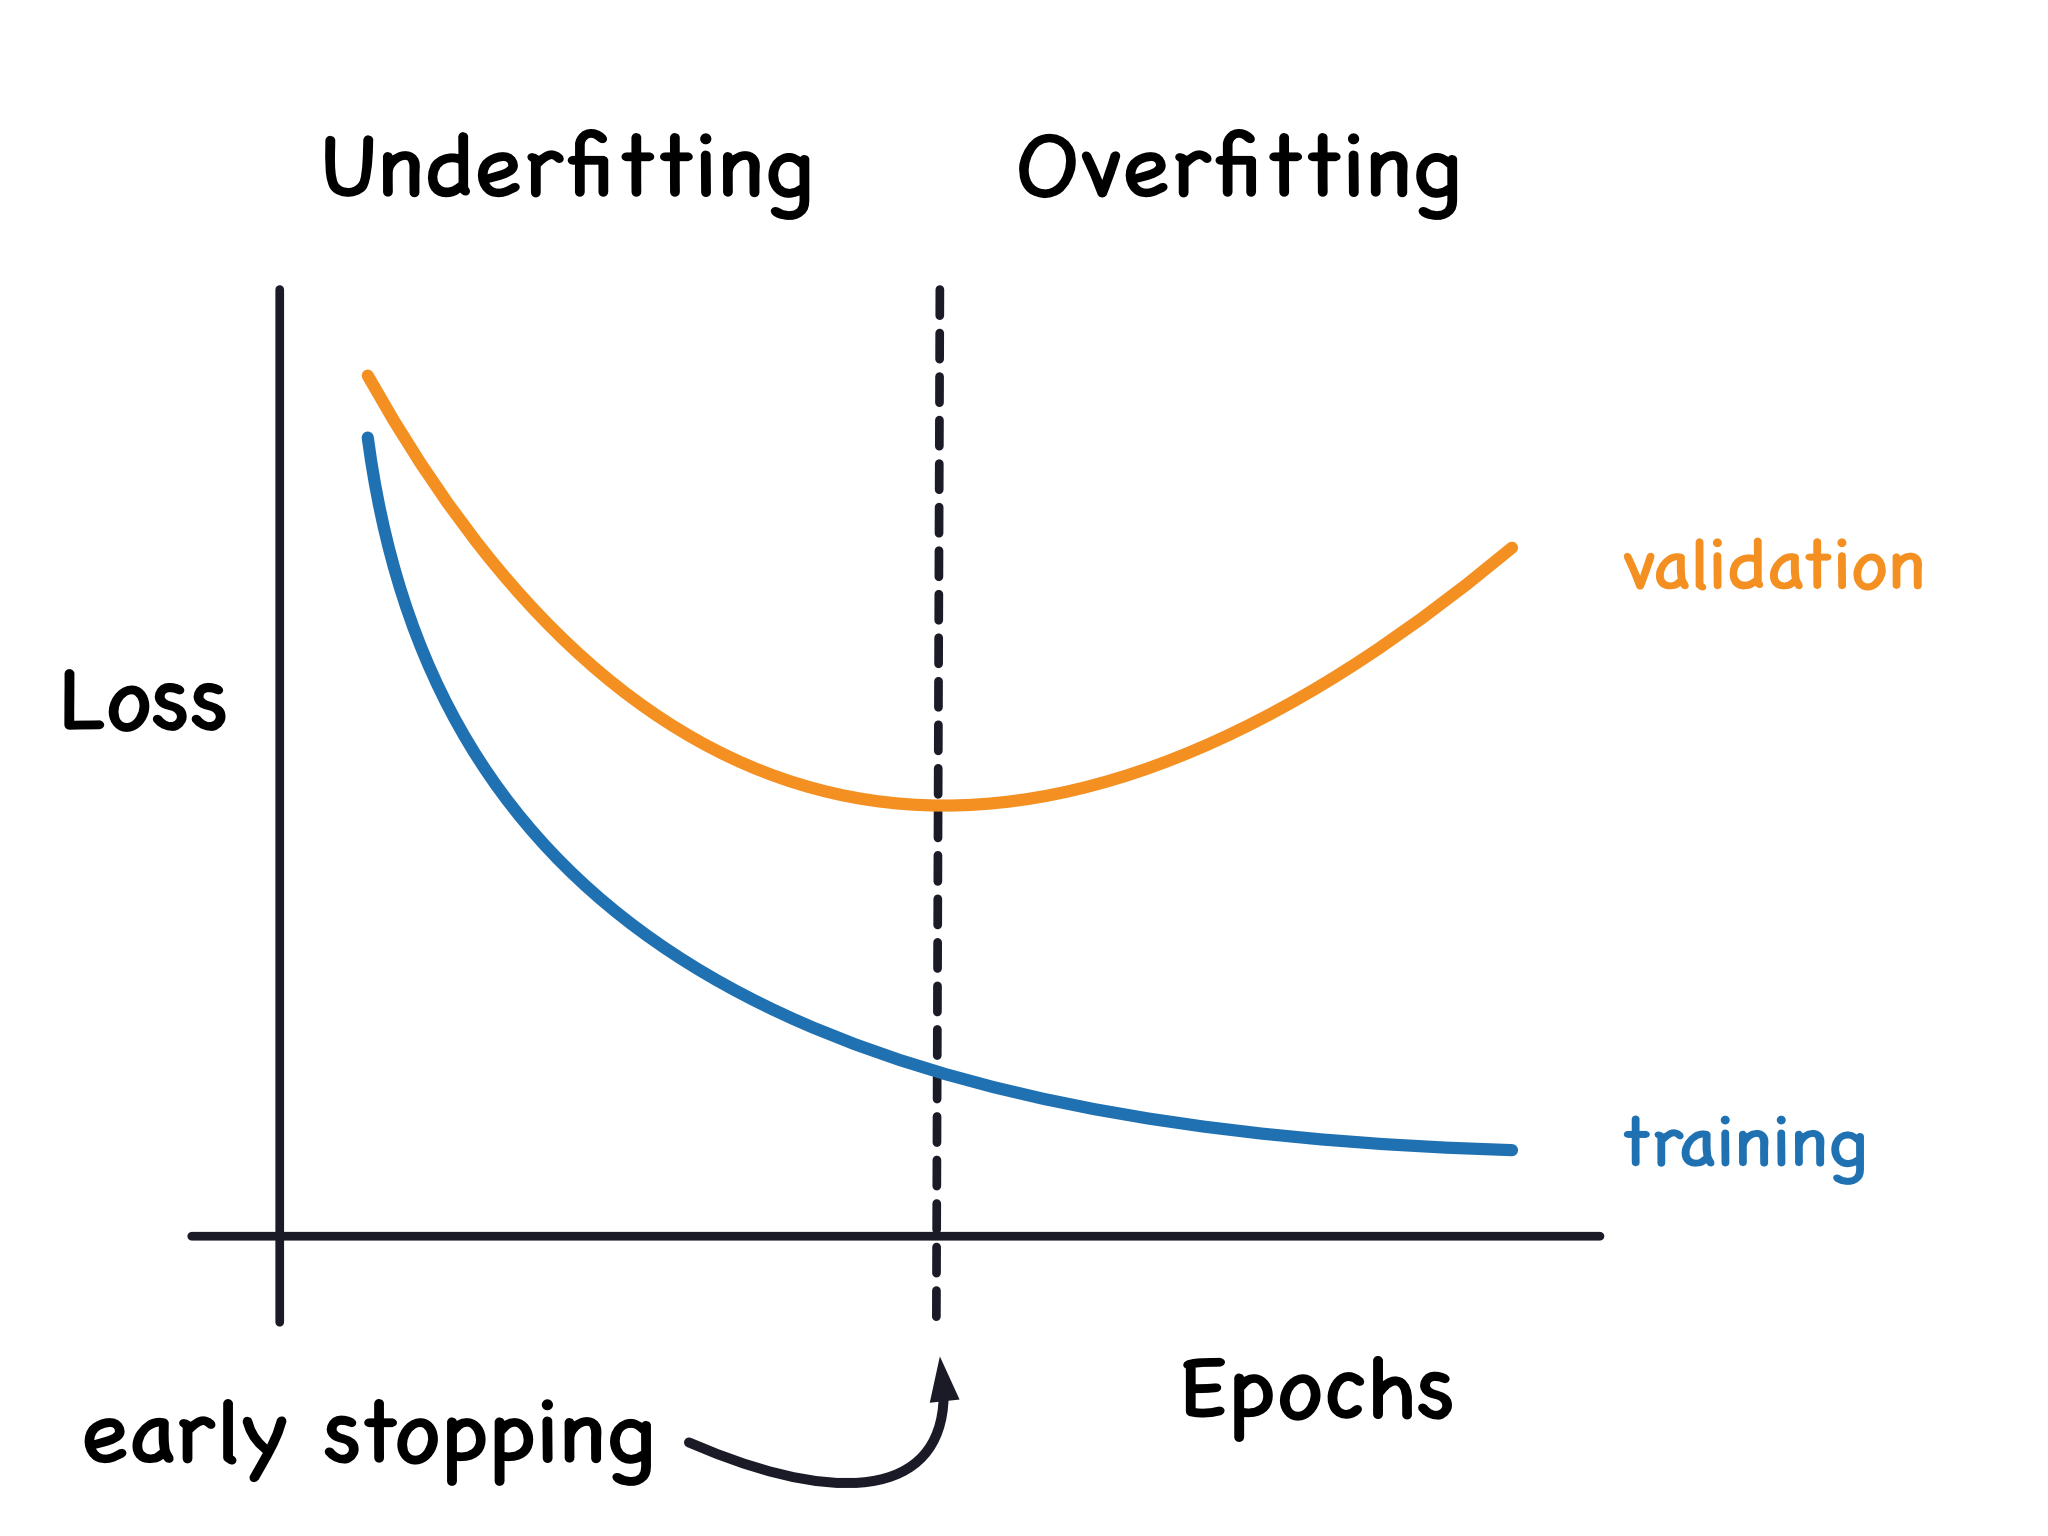
\includegraphics[width=0.45\textwidth]{pic/Early-Stopping.png}
                 % \caption{}
                \label{fig:Early-Stopping}
            \end{figure}
            
    \end{itemize}
\end{frame}
\begin{frame}{Background and Motivation for Dropout}
    \begin{itemize}
        \item \textbf{Ensemble Learning}
            \begin{itemize}
                \item Combines \textbf{multiple models} to increase model capacity and reduce overfitting.
                \item However, training multiple large models can be computationally \textbf{expensive}.
            \end{itemize}
        \item \textbf{Bayesian Regularization}
            \begin{itemize}
                \item Assumes a \textbf{prior distribution} on parameters, balancing data fit with model complexity.
                \item Prevents overfitting by \textbf{limiting model reliance} on specific parameter values.
            \end{itemize}
        \item \textbf{Inspiration from Nature}
            \begin{itemize}
                \item In evolution, genes are mixed randomly in each generation, creating robust organisms by avoiding dependency on specific gene combinations.
                \item Similarly, dropout \textbf{reduces neural dependencies}, encouraging robust, generalizable features.
            \end{itemize}
    \end{itemize}
\end{frame}

\begin{frame}{Concept of Dropout}
    \begin{itemize}
        \item Dropout is a regularization technique that reduces overfitting in neural networks.
        \begin{itemize}
            \item \textbf{Randomly deactivates} neurons in each layer during training.
            \item Effectively trains \textbf{multiple “thinned” sub-networks}, then averages them at test time.
        \end{itemize}
        \item This makes neurons more robust, as they cannot rely on specific other neurons to perform well.
    \end{itemize}
    \begin{figure}
            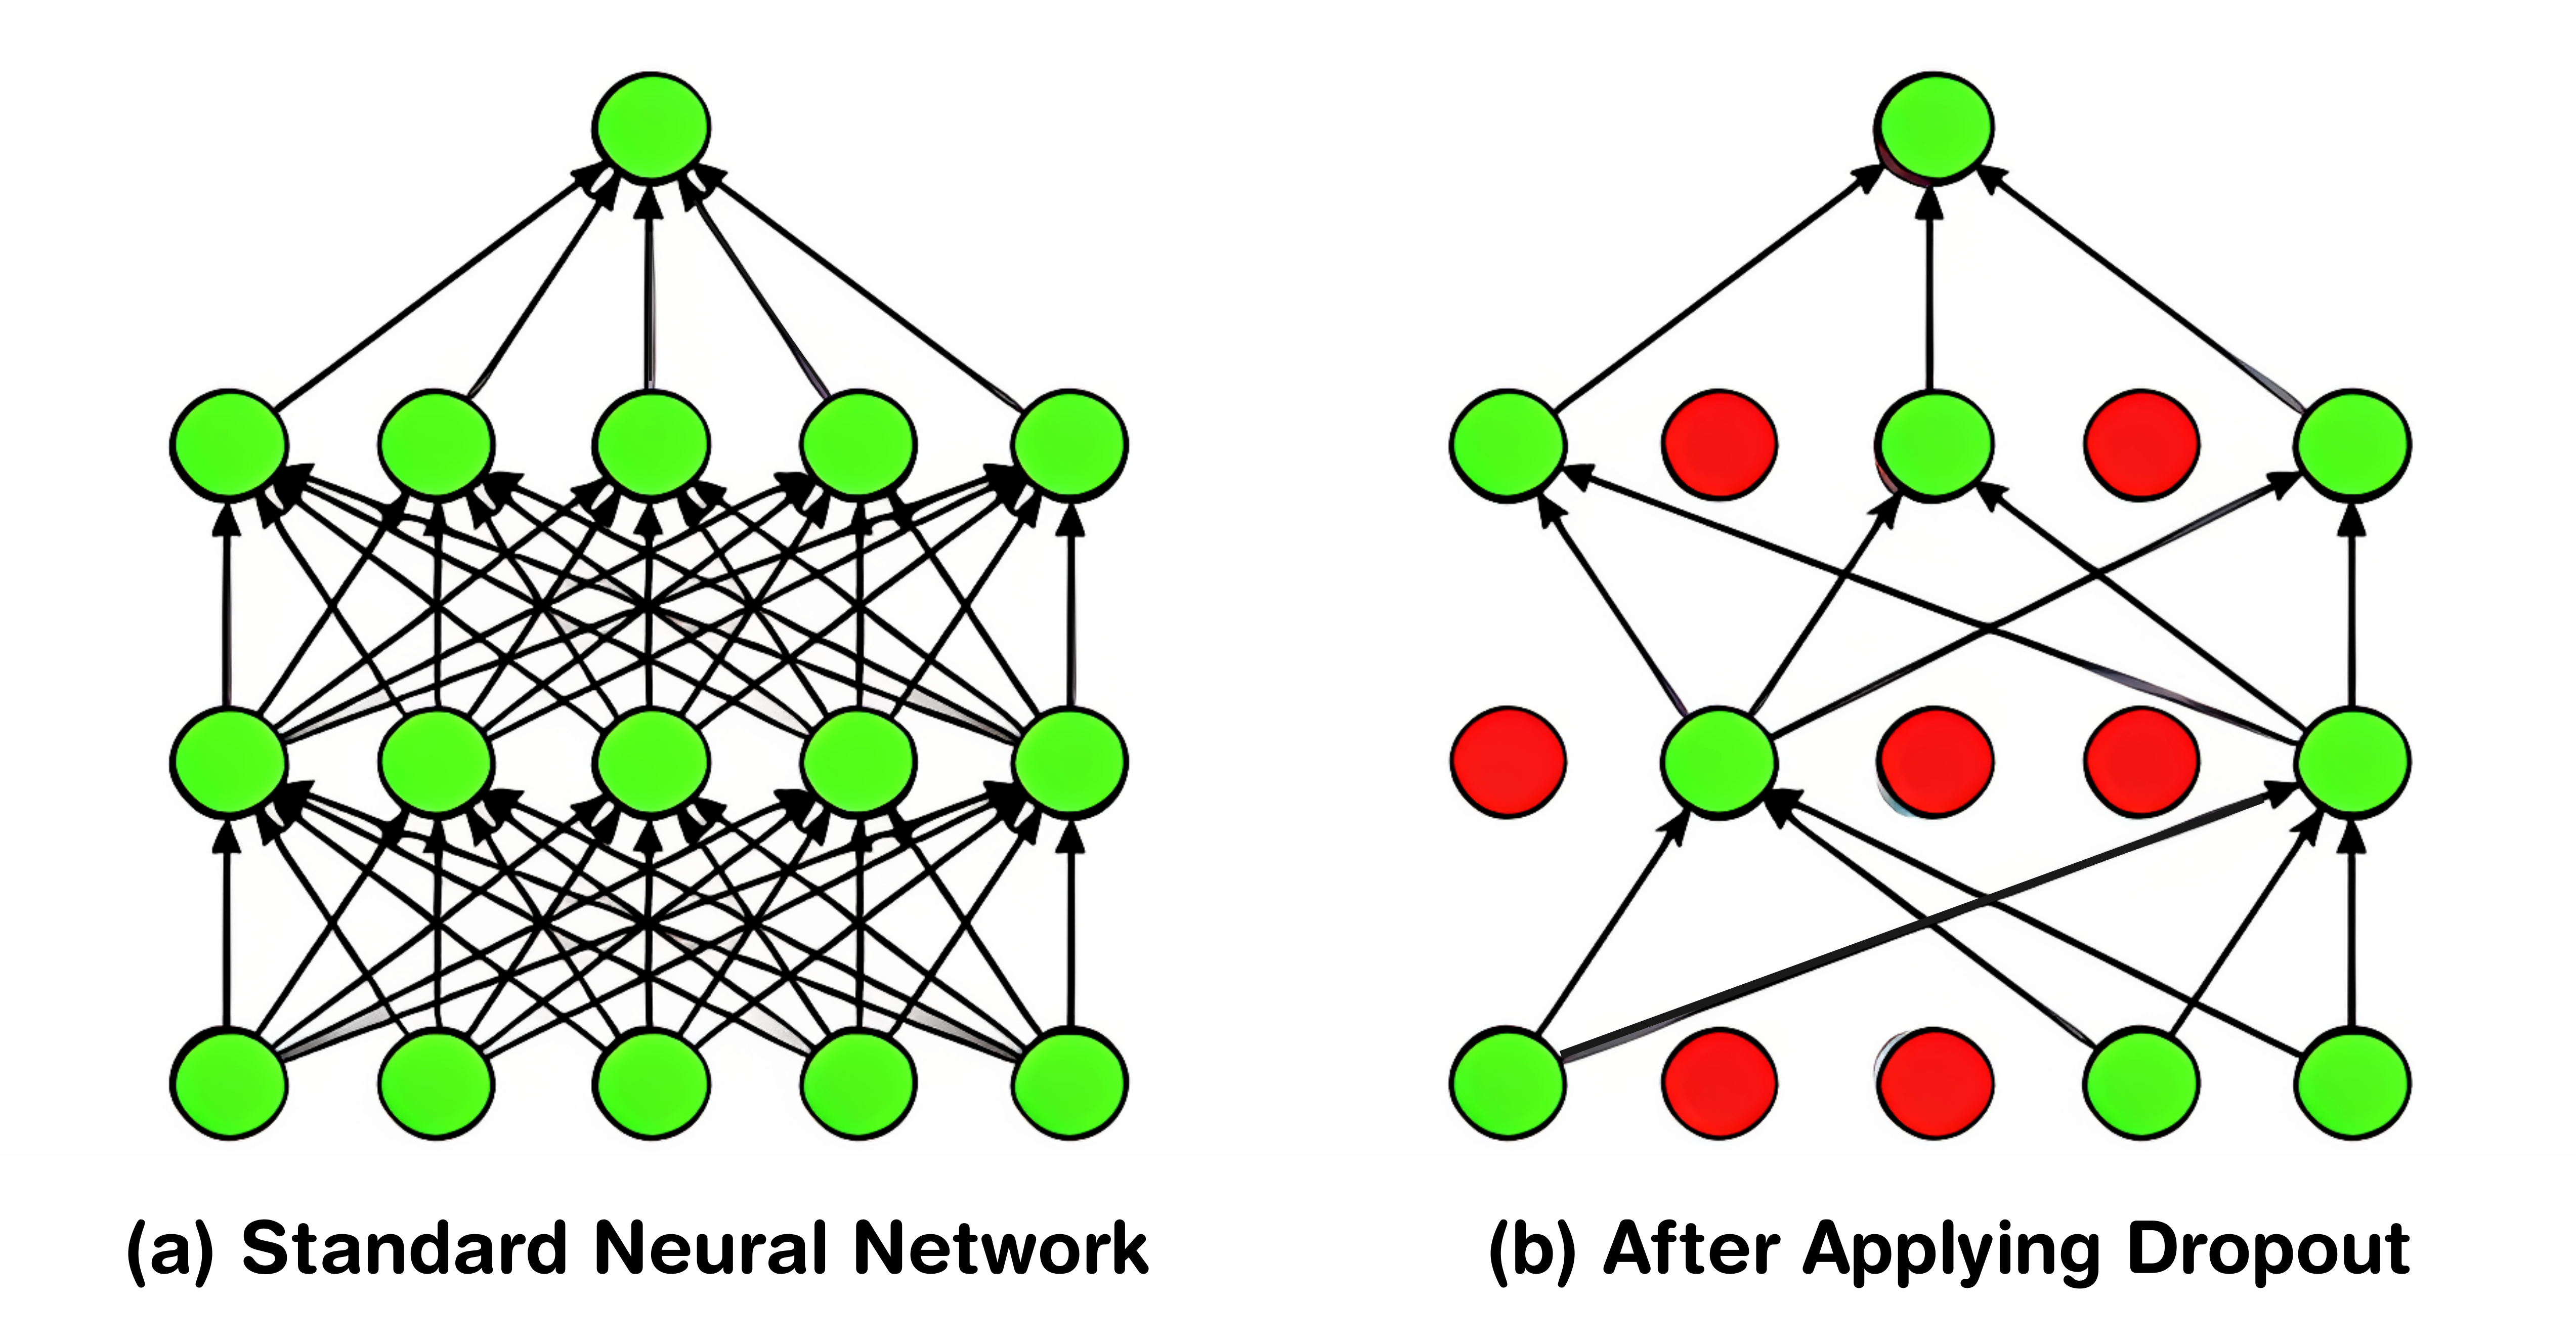
\includegraphics[width=0.6\textwidth]{pic/Dropout.png}
            \label{fig:Dropout}
        \end{figure}
\end{frame}


\begin{frame}{Mechanics of Dropout: Training vs. Inference}
    \begin{columns}
        % Left column for text
        \begin{column}{0.5\textwidth}
            \begin{itemize}
                \item \textbf{During Training}
                \begin{itemize}
                    \item A fraction of neurons is randomly set to zero in each layer (dropout rate typically 0.5 for hidden layers).
                    \item Only \textbf{active neurons} contribute to forward pass and backpropagation.
                \end{itemize}
                \item \textbf{During Inference}
                \begin{itemize}
                    \item All neurons are active.
                    \item To balance the increase in neuron count, \textbf{scale the weights} by the dropout probability.
                    \item Weight scaling compensates for the increase in neuron count, maintaining consistent output expectations.
                \end{itemize}
            \end{itemize}
        \end{column}
        
        % Right column for image
        \begin{column}{0.5\textwidth}
            \begin{figure}
                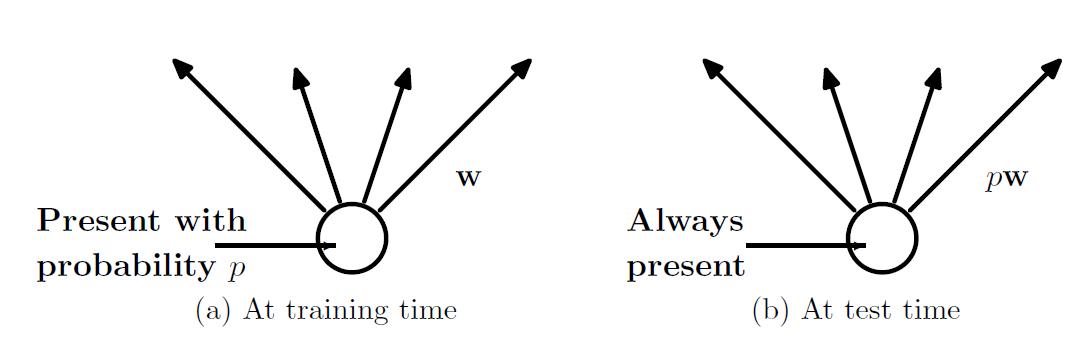
\includegraphics[width=\textwidth]{pic/dropout/test-train.png}
                \caption{Training vs. Inference in Dropout adapted from \href{https://jmlr.org/papers/v15/srivastava14a.html}{Dropout: A Simple Way to Prevent Neural Networks from Overfitting}}
                \label{fig:Dropout}
            \end{figure}
        \end{column}
    \end{columns}
\end{frame}


\begin{frame}{Why Dropout Prevents Overfitting}
    \begin{itemize}
        \item \textbf{Breaks Co-Adaptations}
            \begin{itemize}
                \item Forces neurons to \textbf{operate independently}, creating more generalizable feature representations.
            \end{itemize}
        \item \textbf{Acts as Model Averaging}
            \begin{itemize}
                \item Randomly sampling neuron subsets is akin to training an ensemble of networks.
                \item Inference combines these sub-networks, improving model performance on unseen data.
            \end{itemize}
    \end{itemize}
\end{frame}

\begin{frame}{Real-World Impact of Dropout}
\begin{columns}
    
        \begin{column}{0.5\textwidth}
    \begin{itemize}
        \item \textbf{Applications in Image Recognition}
            \begin{itemize}
                \item Enhanced performance on MNIST, CIFAR-10, and ImageNet, helping models generalize to varied visual inputs.
            \end{itemize}
        \item \textbf{Speech Recognition and Text Classification}
            \begin{itemize}
                \item Reduced error rates on TIMIT speech dataset and improved document classification on Reuters.
            \end{itemize}
        \item \textbf{Computational Biology}
            \begin{itemize}
                \item Used for gene splicing prediction, dropout helps extract robust features from small genetic datasets.
            \end{itemize}
    \end{itemize}
    \end{column}
    \begin{column}{0.5\textwidth}
            \begin{figure}
                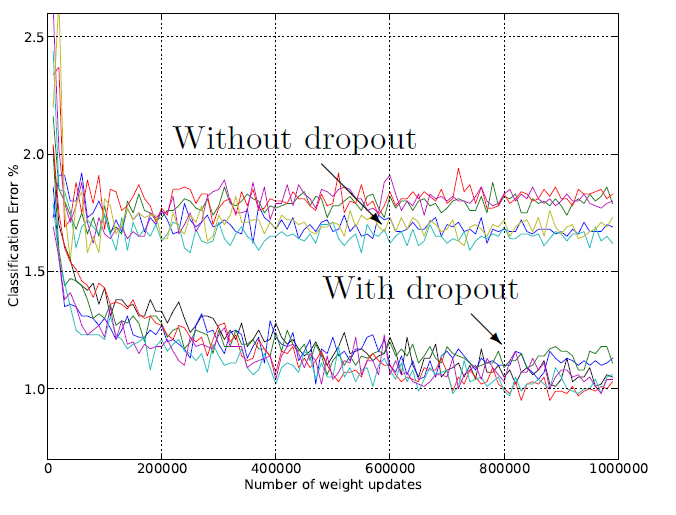
\includegraphics[width=0.9\textwidth]{pic/dropout/effect-of-dropout.png}
                \caption{Effect of dropout for different architectures: adapted from \href{https://jmlr.org/papers/v15/srivastava14a.html}{Dropout: A Simple Way to Prevent Neural Networks from Overfitting}}
                \label{fig:Dropout}
            \end{figure}
        \end{column}
\end{columns}
\end{frame}

\begin{frame}{Dropout Algorithm}
    \begin{figure}
                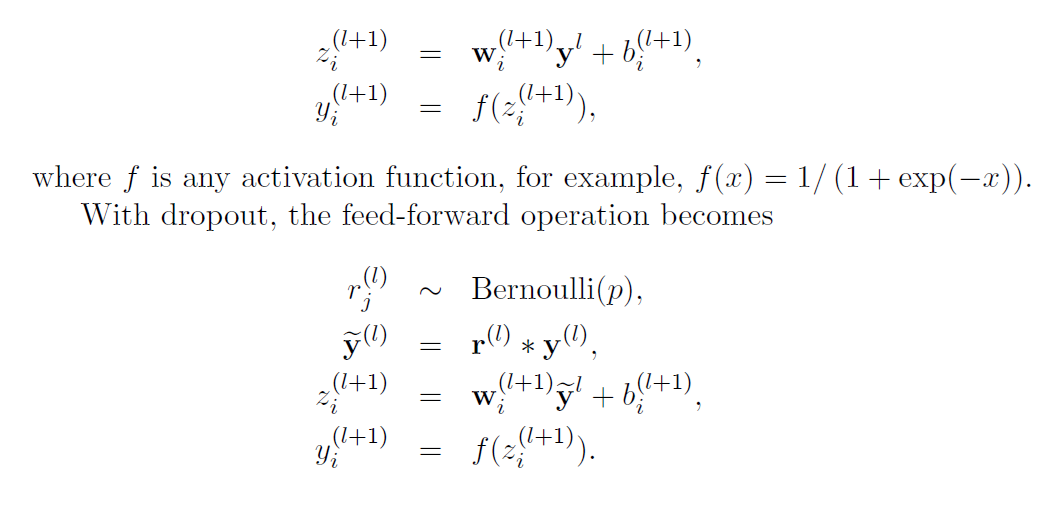
\includegraphics[width=0.8\textwidth]{pic/dropout/algorithm.png}
                \caption{Dropout Algorithm in Feedforward Networks: adapted from \href{https://jmlr.org/papers/v15/srivastava14a.html}{Dropout: A Simple Way to Prevent Neural Networks from Overfitting}}
                \label{fig:Dropout}
            \end{figure}
\end{frame}



\begin{frame}{Dropout Best Practices}
    \begin{itemize}
        \item \textbf{Dropout Rate:} 0.5 for hidden layers is a common starting point, but the rate should be tuned for each model.
        \item \textbf{Where to Apply:} Often applied in fully connected layers; for convolutional layers, spatial dropout is preferred.
        \item \textbf{Avoiding Underfitting:} Avoid using too high of a dropout rate, as this may cause excessive sparsity and underfitting.
    \end{itemize}
\end{frame}




\section{Training Improvements}
% \subsection{Activation Functions}

% \begin{frame}{Activation Functions}
%     \begin{itemize}
%     \item \textbf{Purpose:} Add non-linearity to the network.
%     \item \textbf{Intuition:} Activation functions decide if a neuron should "fire" based on its input, similar to how the brain responds to stimuli.
%     \end{itemize}
% \end{frame}


% \begin{frame}{Activation Functions}
%     \begin{itemize}
%         \item Choosing the right activation function based on the problem.
%         \item Effects on vanishing/exploding gradients.
%         \item Overview of common functions: ReLU, Sigmoid, Tanh, etc.
%     \end{itemize}
% \end{frame}


% \begin{frame}{Different Types of Activation Functions (Part 1)}
%     \centering
%     % \begin{tabular}{|c|c|c|}
%     % \centering
%     \begin{tabular}{|>{\centering\arraybackslash}m{4cm}|>{\centering\arraybackslash}m{5cm}|>{\centering\arraybackslash}m{4cm}|}
%         \hline
%         \textbf{Activation Function} & \textbf{Equation} & \textbf{Plot} \\
%         \hline
%         \textbf{Binary Step} &
%         $\text{Binary Step}(x) = \begin{cases}
%             1 & \text{if } x \geq 0 \\
%             0 & \text{if } x < 0
%         \end{cases}$ &
%         \begin{tikzpicture}[scale=0.35]
%             \begin{axis}[
%                 axis lines=middle,
%                 xlabel={$x$},
%                 ylabel={Binary Step$(x)$},
%                 ymin=-0.5, ymax=1.5,
%                 xmin=-2, xmax=2,
%                 samples=2,
%                 grid=both,
%                 width=6cm,
%                 height=6cm,
%                 ]
%                 \addplot[blue, thick, mark=*] coordinates {(-6, 0) (-0.01, 0) (0, 1) (6, 1)};
%             \end{axis}
%         \end{tikzpicture} \\
%         \hline

%         \textbf{Sigmoid} &
%         $\sigma(x) = \frac{1}{1 + e^{-x}}$ &
%         \begin{tikzpicture}[scale=0.3]
%             \begin{axis}[
%                 axis lines=middle,
%                 xlabel={$x$},
%                 ylabel={$\sigma(x)$},
%                 ymin=-0.1, ymax=1.1,
%                 xmin=-6, xmax=6,
%                 samples=100,
%                 domain=-6:6,
%                 grid=both,
%                 ]
%                 \addplot[green, thick] {1/(1 + exp(-x))};
%             \end{axis}
%         \end{tikzpicture} \\
%         \hline

%         \textbf{Tanh} &
%         $\tanh(x) = \frac{e^x - e^{-x}}{e^x + e^{-x}}$ &
%         \begin{tikzpicture}[scale=0.3]
%             \begin{axis}[
%                 axis lines=middle,
%                 xlabel={$x$},
%                 ylabel={$\tanh(x)$},
%                 ymin=-1.1, ymax=1.1,
%                 xmin=-6, xmax=6,
%                 samples=100,
%                 grid=both,
%                 ]
%                 \addplot[red, thick] {tanh(x)};
%             \end{axis}
%         \end{tikzpicture} \\
%         \hline

%     \end{tabular}
% \end{frame}

% % Second Frame
% \begin{frame}{Different Types of Activation Functions (Part 2)}
%     \centering
%     \begin{tabular}{|>{\centering\arraybackslash}m{4cm}|>{\centering\arraybackslash}m{5cm}|>{\centering\arraybackslash}m{4cm}|}
%         \hline
%         \textbf{Activation Function} & \textbf{Equation} & \textbf{Plot} \\
%         \hline

%         \textbf{ReLU} &
%         $\text{ReLU}(x) = \max(0, x)$ &
%         \begin{tikzpicture}[scale=0.3]
%             \begin{axis}[
%                 axis lines=middle,
%                 xlabel={$x$},
%                 ylabel={ReLU$(x)$},
%                 ymin=-1, ymax=6,
%                 xmin=-6, xmax=6,
%                 samples=100,
%                 grid=both,
%                 ]
%                 \addplot[cyan, thick] {max(0, x)};
%             \end{axis}
%         \end{tikzpicture} \\
%         \hline

%         \textbf{Leaky ReLU} &
%         $\text{Leaky ReLU}(x) = \begin{cases}
%             x & \text{if } x > 0 \\
%             \alpha x & \text{if } x \leq 0
%         \end{cases}$ &
%         \begin{tikzpicture}[scale=0.3]
%             \begin{axis}[
%                 axis lines=middle,
%                 xlabel={$x$},
%                 ylabel={Leaky ReLU$(x)$},
%                 ymin=-2, ymax=6,
%                 xmin=-6, xmax=6,
%                 samples=100,
%                 grid=both,
%                 ]
%                 \pgfmathsetmacro{\alpha}{0.1}
%                 \addplot[orange, thick] {x > 0 ? x : \alpha*x};
                
%             \end{axis}
%         \end{tikzpicture} \\
%         \hline

%         \textbf{ELU} &
%         $\text{ELU}(x) = \begin{cases}
%             x & \text{if } x > 0 \\
%             \alpha (e^x - 1) & \text{if } x \leq 0
%         \end{cases}$ &
%         \begin{tikzpicture}[scale=0.3]
%             \begin{axis}[
%                 axis lines=middle,
%                 xlabel={$x$},
%                 ylabel={ELU$(x)$},
%                 ymin=-2, ymax=6,
%                 xmin=-6, xmax=6,
%                 samples=100,
%                 grid=both,
%                 ]
%                 \addplot[purple, thick] {x > 0 ? x : 1*(exp(x) - 1)};
%             \end{axis}
%         \end{tikzpicture} \\
%         \hline

%     \end{tabular}
% \end{frame}

% \subsection{Weight Initialization}

% \begin{frame}{Key Initialization Techniques}
%     \begin{itemize}
%         \item \textbf{Zero Initialization:} Set all weights to zero (rarely used).
%         \item \textbf{Random Initialization:} Assign small random values to weights.
%         \item \textbf{Xavier Initialization:} Scales weights based on the number of neurons to maintain variance across layers.
%         \item \textbf{He Initialization:} Optimized for ReLU activation functions, scales weights to prevent vanishing/exploding gradients.
%         \item Prevent vanishing/exploding gradients with proper initialization.
%     \end{itemize}
% \end{frame}


\subsection{Hyperparameter Tuning}

\begin{frame}{Introduction to Hyperparameter Tuning}
    \begin{itemize}
        \item \textbf{Definition:} Hyperparameters are settings external to the model that control the training process and model capacity. They cannot be learned from the data.
        \item \textbf{Examples:} Learning rate, batch size, number of layers, number of neurons per layer, dropout rate, etc.
        \item \textbf{Impact:} Choosing the right hyperparameters can significantly enhance model performance, while poor choices may cause underfitting or overfitting.
    \end{itemize}
\end{frame}


\begin{frame}{Why Hyperparameter Tuning Matters}
    \begin{itemize}
        \item \textbf{Optimization Goal:} Identify the hyperparameters that maximize model performance on validation data.
        \item \textbf{Challenges:}
            \begin{itemize}
                \item Large, high-dimensional search space.
                \item High computational cost due to repeated training and evaluation.
                \item Noisy objective function – performance can vary due to randomness (e.g., weight initialization).
            \end{itemize}
        \item \textbf{Trade-offs:} Balancing computation time with model performance.
    \end{itemize}
\end{frame}


\begin{frame}{Approaches to Hyperparameter Tuning}
    \begin{itemize}
        \item \textbf{Grid Search:} An exhaustive search over a predefined set of hyperparameter combinations.
        \item \textbf{Random Search:} Randomly samples hyperparameters, sometimes finding good configurations more efficiently than grid search.
    \end{itemize}
    \begin{figure}
        \centering
        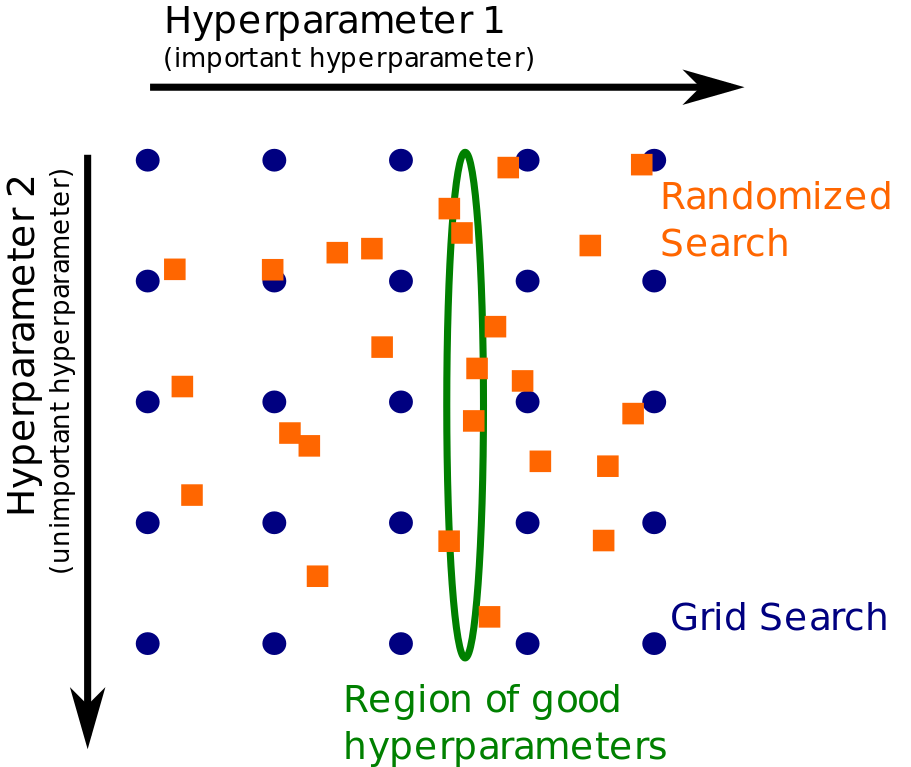
\includegraphics[width=0.3\textwidth]{pic/grid_vs_random_search.png}
        \caption{Grid Search vs. Random Search in Hyperparameter Tuning.}
        \label{fig:hyperparameter_tuning}
    \end{figure}
\end{frame}

\begin{frame}{Hyperparameter Tuning Best Practices}
    \begin{itemize}
        \item \textbf{Start Simple:} Begin with tuning a smaller subset of key hyperparameters (e.g., learning rate, batch size).
        \item \textbf{Use Cross-Validation:} Instead of a single validation set, use techniques like k-fold cross-validation to ensure performance is not dependent on a specific train-validation split.
        \item \textbf{Automate:} Leverage frameworks like \texttt{scikit-learn} to automate and parallelize the tuning process.
        \item \textbf{Track Experiments:} Use tools like \texttt{Wandb} to systematically track hyperparameters, training metrics, and results.
        \item \textbf{Use Learning Curves:} Plot learning curves to monitor the model's performance over time and detect overfitting or underfitting early.
        \item \textbf{Budget Time and Resources:} Set limits on tuning (e.g., time, number of iterations) to avoid excessive computational costs.
    \end{itemize}
\end{frame}



\subsection{Monitoring Training Process}

\begin{frame}{Monitoring Training Process}
    \begin{itemize}
        \item Track key metrics: Loss, accuracy, validation loss.
        \item Use \texttt{wandb} for real-time monitoring and logging.
        \item Wandb Panels: visualizations to explore your logged data, the relationships between hyperparameters and output metrics, and dataset examples.
        \item Detect overfitting early by analyzing trends in training and validation metrics.
        \item Visualize progress using learning curves to assess model performance over time.
    \end{itemize}
    \begin{figure}
        \centering
        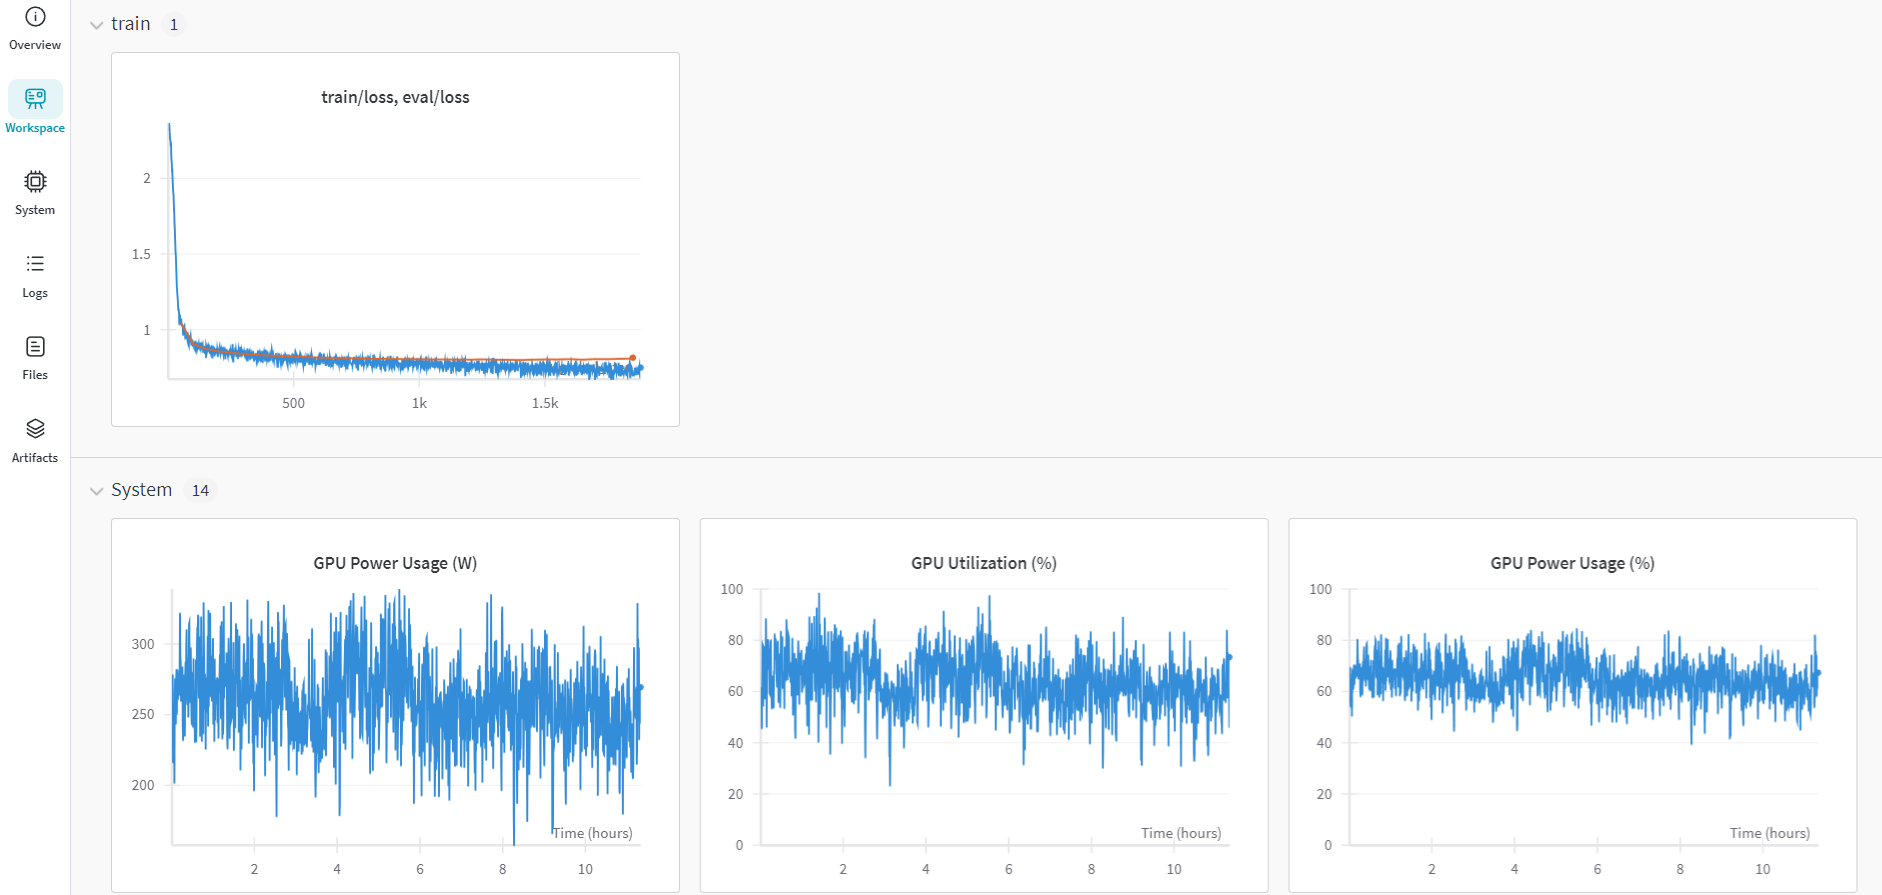
\includegraphics[width=0.5\textwidth]{pic/wandb.png}
        \caption{Training metrics visualization in \texttt{wandb}.}
        \label{fig:wandb}
    \end{figure}
\end{frame}



% \section{Batch Normalization}
% \subsection{Why Batch Normalization?}
% \subsection{How Batch Normalization Works}
% \subsection{Advantages and Disadvantages of Batch Normalization}
% \subsection{Batch Normalization in Practice}
% \subsection{Closing Takeaways on Batch Normalization}


\section{References}

\begin{frame}[allowframebreaks]
    \bibliography{ref}
    \bibliographystyle{ieeetr}
    \nocite{*} % used here because no citation happens in slides
    % if there are too many try use:
    % \tiny\bibliographystyle{alpha}
\end{frame}

\begin{frame}{Contributions}
	\textbf{These slides are authored by:}
	\begin{itemize}
 		\item Faezeh Sarlakifar
		\item Sogand Salehi
	\end{itemize}
	    
\end{frame}
\begin{frame}
    \begin{center}
        {\Huge Any Questions?}
    \end{center}
\end{frame}

\end{document}
